\section{Background}\label{sec-background}

Build systems automate the execution of simple repeatable tasks for individual
users, as well as for large organisations. In this section we explore the design
space of build systems, using four concrete examples:
\Make~\cite{feldman1979make}, \Shake~\cite{mitchell2012shake},
\Bazel~\cite{bazel}, and \Excel~\cite{advanced_excel}\footnote{\Excel appears
very different to the others but, seen through the lens of this paper, it is
very close indeed.}.
We have carefully chosen these four to illustrate the various axes on which build systems
differ; we discuss many other notable examples
of build systems, and their relationships,
in~\S\ref{sec-related}.

\subsection{The venerable \Make: static dependencies and file modification times}
\label{sec-background-make}

\Make\footnote{There are numerous implementations of \Make and none comes with a
formal specification. In this paper we therefore use a simple and sensible
approximation to a real \Make that you might find on your machine.} was developed
more than 40 years ago to automatically build software libraries and executable
programs from source code. It uses \emph{makefiles} to describe tasks (often
referred to as \emph{build rules}) and their dependencies in a simple textual form.
For example\footnote{Do not worry about the dependency on \cmd{stdio.h}, and
its transitive (perhaps dynamic) dependencies.
We will deal with these in Section~\S\ref{sec-task-monad}.}:

\vspace{1mm}
\begin{minted}[xleftmargin=10pt]{makefile}
util.o: util.h util.c
    gcc -c util.c
\end{minted}
\vspace{1mm}
\begin{minted}[xleftmargin=10pt]{makefile}
main.o: util.h main.c
    gcc -c main.c
\end{minted}
\vspace{1mm}
\begin{minted}[xleftmargin=10pt]{makefile}
main.exe: util.o main.o
    gcc util.o main.o -o main.exe
\end{minted}
\vspace{1mm}

\noindent
The above makefile lists three tasks: (i) compile a utility library comprising
files \cmd{util.h} and \cmd{util.c} into \cmd{util.o} by
executing\footnote{In this example we pretend \cmd{gcc} is a pure function for the
sake of simplicity. In reality, there are multiple versions of \cmd{gcc} and the
actual binary that is used to compile and link files is often also listed as a task
dependency.} the command \cmd{gcc -c util.c}, (ii) compile the main source file
\cmd{main.c} into \cmd{main.o}, and (iii) link object files \cmd{util.o} and
\cmd{main.o} into the executable \cmd{main.exe}. The makefile contains the
complete information about the \emph{task dependency graph}, which is shown in
Fig.~\ref{fig-make}(a).

\begin{figure}[h]
\begin{subfigure}[b]{0.32\linewidth}
\centerline{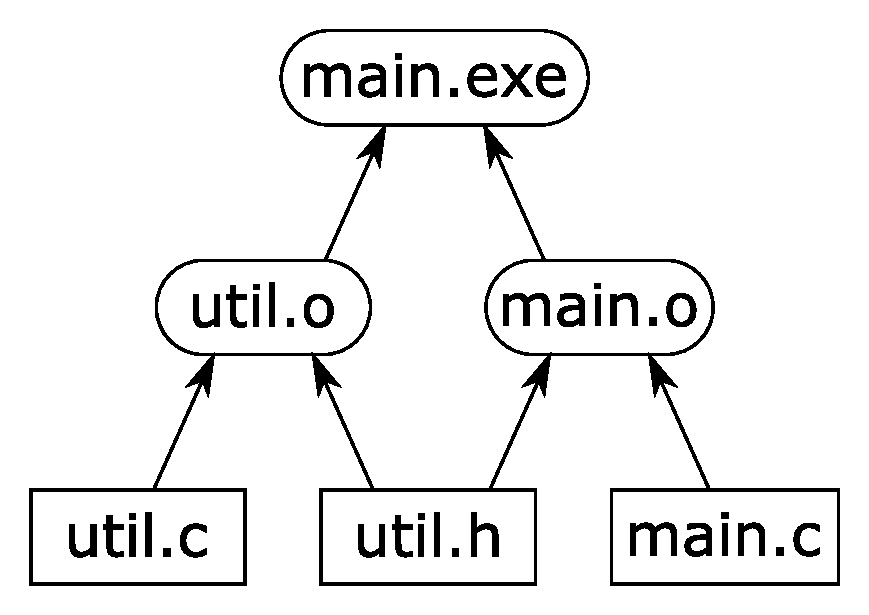
\includegraphics[scale=0.28]{fig/make-example.pdf}}
\caption{Task dependency graph}
\end{subfigure}
\begin{subfigure}[b]{0.32\linewidth}
\centerline{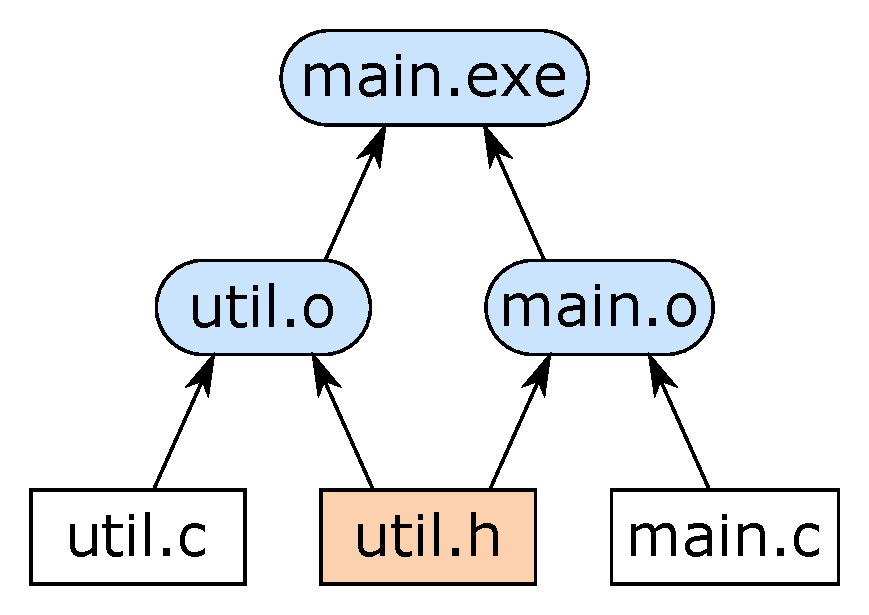
\includegraphics[scale=0.28]{fig/make-example-full.pdf}}
\caption{Full rebuild}
\end{subfigure}
\begin{subfigure}[b]{0.32\linewidth}
\centerline{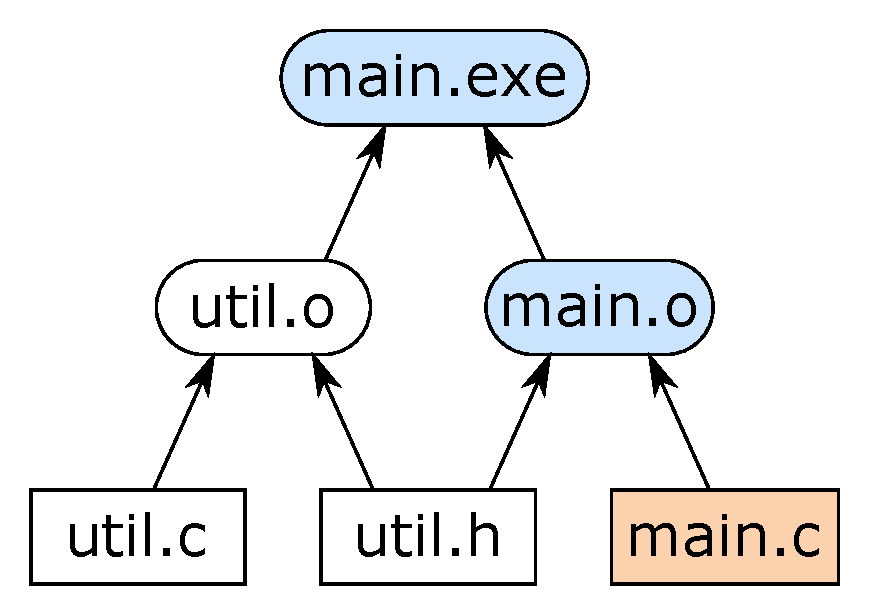
\includegraphics[scale=0.28]{fig/make-example-partial.pdf}}
\caption{Partial rebuild}
\end{subfigure}
\vspace{-2mm}
\caption{A task dependency graph and two build scenarios. Input files are shown
as rectangles, intermediate and output files are shown as rounded rectangles.
Modified inputs and files that are rebuilt are highlighted.
\label{fig-make}}
\vspace{-2mm}
\end{figure}

If the user runs \Make specifying \cmd{main.exe} as the desired output, \Make
will first build \cmd{util.o} and \cmd{main.o}, in any order since these
tasks are independent, and then build \cmd{main.exe}. If the
user modifies the sources of \cmd{util.h} and runs \Make again, it will
perform a \emph{full rebuild}, because all three tasks transitively depend on
\cmd{util.h}, as illustrated in Fig.~\ref{fig-make}(b). On the other hand, if
the user modifies \cmd{main.c} then a \emph{partial rebuild} is sufficient:
the file \cmd{util.o} does not need to be rebuilt, since its inputs have not
changed, see Fig.~\ref{fig-make}(c). Note that if the dependency graph is
\emph{acyclic} then each task needs to be executed at most once. Cyclic task
dependencies are typically not allowed in build systems although there are rare
exceptions, see~\S\ref{sec-iterative-compute}.

The following property is essential for build systems; indeed, it is their raison d'\^etre:

\definition[Minimality]{A build system is \emph{minimal} if it executes tasks at
most once per build and only if they transitively depend on inputs that changed
since the previous build.}\label{def-minimal}
\vspace{2mm}

To achieve minimality \Make relies on two main ideas: (i) it uses \emph{file
modification time} to detect which files changed\footnote{Technically, you
can fool \Make by altering the modification time of a file without changing its
content, e.g. by using the command \cmd{touch}. \Make is therefore minimal only
under the assumption that you do not do that.}, and (ii) it constructs a task
dependency graph from the information contained in the makefile and executes
tasks in a \emph{topological order}. For a more concrete description
see~\S\ref{sec-implementation-make}.

\subsection{\Excel: dynamic dependencies at the cost of minimality}
\label{sec-background-excel}

\Excel is a build system in disguise. Consider the following simple spreadsheet.

\vspace{1mm}
\begin{minted}[xleftmargin=10pt]{text}
A1: 10      B1: A1 + A2
A2: 20
\end{minted}
\vspace{1mm}

\noindent
There are two input cells \cmd{A1} and \cmd{A2}, and a single task that computes
the sum of their values, writing the result into the cell \cmd{B1}. If either of
the inputs change, \Excel will recompute the result.

Unlike \Make, \Excel does not need to know all task dependencies upfront. Some
dependencies may change \emph{dynamically} according to computation results. For
example:

\vspace{1mm}
\begin{minted}[xleftmargin=10pt]{text}
A1: 10      B1: INDIRECT("A" & C1)      C1: 1
A2: 20
\end{minted}
\vspace{1mm}

\noindent
The formula in \cmd{B1} uses the \cmd{INDIRECT} function, which takes a string and
returns the value of the cell with that name.  The string evaluates
to \cmd{"A1"}, so \cmd{B1} evaluates to \cmd{10}. However, the dependencies of the
formula in \cmd{B1} are determined by the value of \cmd{C1}, so there is no
possibility\footnote{In this particular example one might say that
the value of \cmd{C1} is statically known, but imagine that it is the result of a long computation
chain -- its value will only become available during the build.}
of computing the dependency graph prior to calc.

To support dynamic dependencies,
\Excel's build algorithm~\cite{excel_recalc} is significantly different from
\Make. \Excel uses the \emph{calculation chain}
produced by the previous build as an approximation to the correct topological
order. During recalculation, \Excel processes cells in this order, but can
\emph{defer recalculation of a cell} by moving it down the chain if a newly
discovered dependency has not yet been rebuilt. We refer to this
algorithm as \emph{restarting}, and will discuss it in more detail
in~\S\ref{sec-implementation-excel}.

Dynamic dependencies complicate minimality.  In the above example, \cmd{B1}
should only be recomputed if \cmd{A1} or \cmd{C1} change, but not if (say)
\cmd{A2} changes; but these facts are not statically apparent. In practice
\Excel implements a conservative approximation to minimality: roughly, it
recomputes a formula if (i) the formula text mentions a changed cell, or (ii)
the formula uses a function like \cmd{INDIRECT} whose dependencies are not
statically visible.

Another distinguishing feature of \Excel is \emph{self-tracking}. Most build
systems only track changes of inputs and intermediate results, but \Excel can
also track changes in the tasks themselves: if a formula is modified, \Excel
will recompute it and propagate the changes. Self-tracking is uncommon in
software build systems, where one often needs to manually initiate a full
rebuild even if just a single build task has changed. We discuss
self-tracking further in~\S\ref{sec-tracking-aspects}.

\begin{figure}[h]
\vspace{-2mm}
\begin{subfigure}[b]{0.90\linewidth}
\centerline{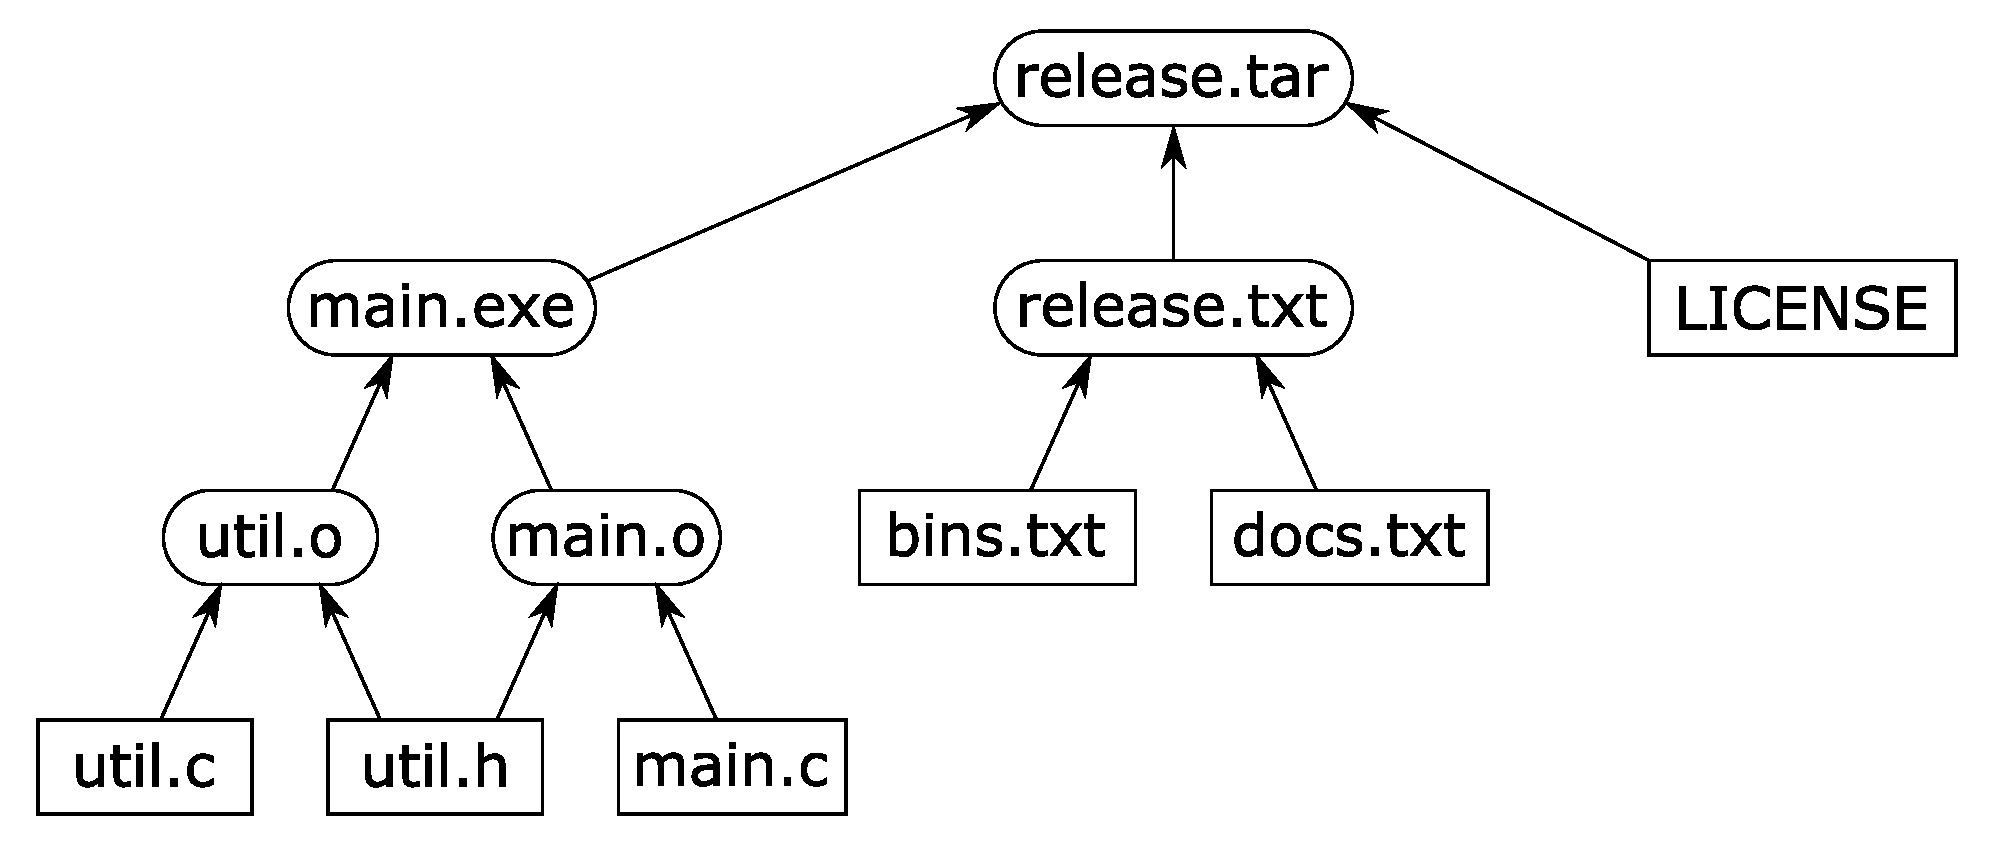
\includegraphics[scale=0.28]{fig/shake-example.pdf}}
\caption{Dependency graph produced after the previous build.}
\end{subfigure}
\begin{subfigure}[b]{0.90\linewidth}
\centerline{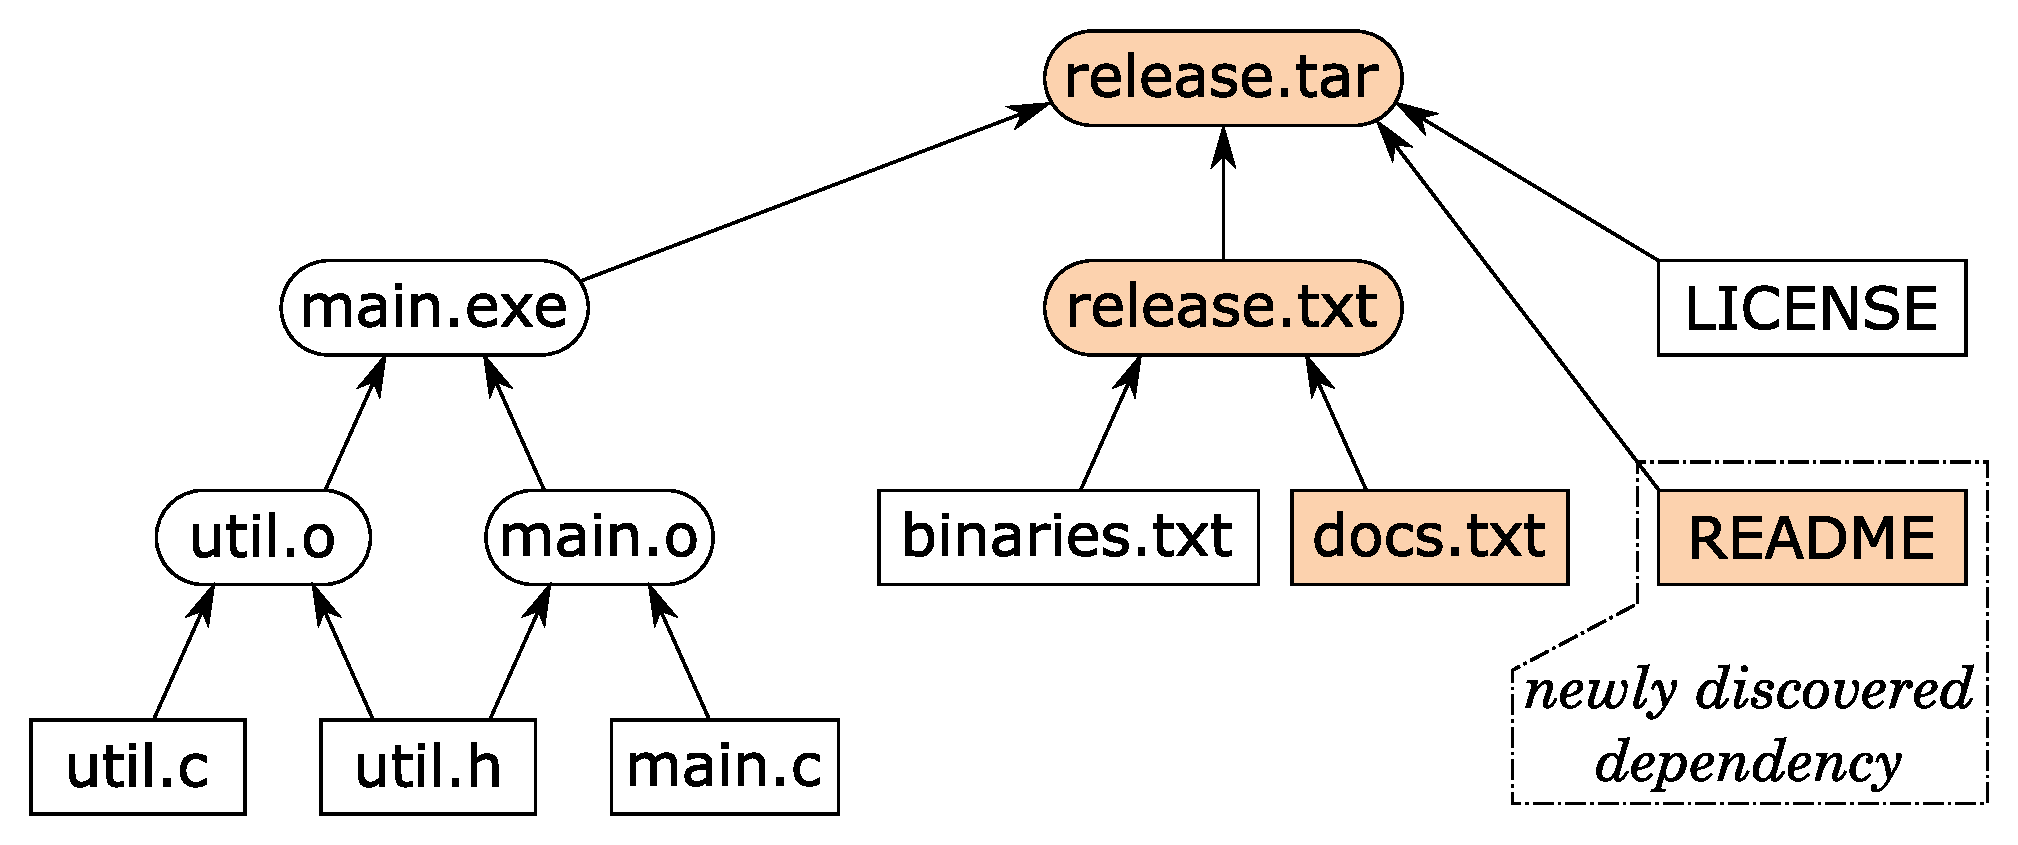
\includegraphics[scale=0.28]{fig/shake-example-rebuild.pdf}}
\caption{Since \cmd{docs.txt} was modified, we rebuild \cmd{release.txt} and
\cmd{release.tar}, discovering a new dependency.}
\end{subfigure}
\vspace{-2mm}
\caption{Dynamic dependencies example: create \cmd{README} and add it to the
list of release documents \cmd{docs.txt}.\label{fig-shake}}
\vspace{-4mm}
\end{figure}

\subsection{\Shake: dynamic dependencies with no remorse}
\label{sec-background-shake}

\Shake was developed to solve the issue of dynamic
dependencies~\cite{mitchell2012shake} without sacrificing
the minimality requirement. Building on the \Make example
from~\S\ref{sec-background-make}, we add the following files whose
dependencies are shown in Fig.~\ref{fig-shake}(a):

\begin{itemize}
    \item \cmd{LICENSE} is an input text file containing the project license.
    \item \cmd{release.txt} is a text file listing all files that should be in the release. This file
    is produced by concatenating input files \cmd{bins.txt} and \cmd{docs.txt}
    that list all binary and documentation files of the project.
    \item \cmd{release.tar} is the release archive built by executing the
    command \cmd{tar} on the release files.
\end{itemize}

The dependencies of \cmd{release.tar} are not known statically: they are
determined by the content of \cmd{release.txt}, which might not even exist
before the build. Makefiles cannot express such dependencies, requiring problematic
workarounds such as \emph{build phases} \cite{hadrian}.
In \Shake we can express the rule for \cmd{release.tar} as:

\begin{minted}[xleftmargin=10pt]{haskell}
"release.tar" %> \_ -> do
    need ["release.txt"]
    files <- lines <$> readFile "release.txt"
    need files
    system "tar" $ ["-cf", "release.tar"] ++ files
\end{minted}

\noindent
We first declare the static dependency on \cmd{release.txt}, then read its
content (a list of files) and depend on each listed file, dynamically. Finally, we specify the
command to produce the resulting archive. Crucially, the archive will only be
rebuilt if one of the dependencies (static or dynamic) has changed. For example,
if we create another documentation file \cmd{README} and add it to
\cmd{docs.txt}, \Shake will appropriately rebuild \cmd{release.txt} and
\cmd{release.tar}, discovering the new dependency, see Fig.~\ref{fig-shake}(b).

\Shake's implementation is different from both \Make and \Excel in two aspects.
First, it uses the dependency graph from the previous build to decide which
files need to be rebuilt. This idea has a long history, going back to
\emph{incremental}~\cite{demers1981incremental},
\emph{adaptive}~\cite{acar2002adaptive}, and
\emph{self-adjusting computations} (see \cite{acar2007selfadjusting} and \S\ref{sec-related}).
Second, instead of abandoning
and deferring the execution of tasks whose newly discovered dependencies have
not yet been built (as \Excel does), \Shake \emph{pauses} their execution until
the dependencies are brought up to date. We refer to this build algorithm as
\emph{recursive}.

\begin{figure}[h]
\vspace{-5mm}
\centerline{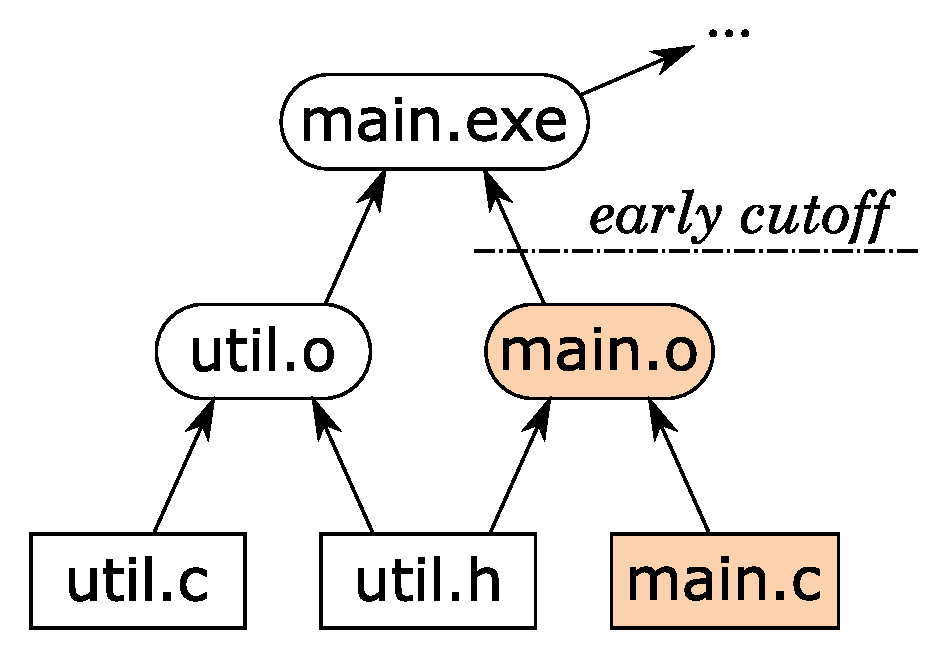
\includegraphics[scale=0.28]{fig/shake-example-cutoff.pdf}}
\vspace{-3mm}
\caption{An early cutoff example: if a comment is added to \cmd{main.c}, the
rebuild is stopped after detecting that \cmd{main.o} is unchanged, since this
indicates that \cmd{main.exe} and its dependents do not need to be
rebuilt.\label{fig-cutoff}}
\vspace{-2mm}
\end{figure}

\Shake also supports the \emph{early cutoff optimisation}. When it
executes a task and the result is unchanged from the previous build, it is
unnecessary to execute the dependent tasks, and hence \Shake can stop a build
earlier, as illustrated in Fig.~\ref{fig-cutoff}. Not all build systems support
early cutoff: \Make and \Excel do not, whereas \Shake and \Bazel (introduced
below) do.

\subsection{\Bazel: a cloud build system}
\label{sec-background-bazel}

When build systems are used by large teams, different team members often end up
executing exactly the same tasks on their local machines. A \emph{cloud build
system} can speed up builds dramatically by sharing build results
among team members. Furthermore, cloud build systems allow one to perform
\emph{shallow builds} that materialise only end build products locally, leaving
all intermediates in the cloud. We illustrate shallow cloud builds by an example
in Fig.~\ref{fig-bazel}.

The user starts by checking out the project sources, whose hashes are (for
simplicity)~1,~2~and~3, and requests to build \cmd{main.exe}, see
Fig.~\ref{fig-bazel}(a,b). By looking up the global history of all previous
builds of the project\footnote{Here we ignore the issue of limited cloud storage
resources for the sake of simplicity; in practice, old entries are regularly
evicted from the storage, as further discussed in~\S\ref{sec-cloud-aspects}.},
the build system finds that someone has already compiled these exact sources
before and their resulting files \cmd{util.o} and \cmd{main.o} had hashes 4~and~5.
Similarly, the build system finds that the hash of the resulting \cmd{main.exe}
should be 6 and downloads the actual binary from the shared cloud storage, since
it is the end build product and must therefore be materialised.

In the second scenario, shown in Fig.~\ref{fig-bazel}(c), the user modifies the
source \cmd{util.c}, thereby changing its hash from~1~to~7. The build system
finds that nobody has ever compiled the new $\{\cmd{util.c}, \cmd{util.h}\}$
combination and must therefore build \cmd{util.o}, which results in changing its
hash from~4~to~8. The combination of hashes of \cmd{util.o} and
\cmd{main.o} has not been encountered before either, therefore the build system
first downloads \cmd{main.o} from the cloud and then builds \cmd{main.exe} by
linking the two object files. When the build is complete, the results
can be uploaded to the cloud for future reuse by other team members.

\Bazel is one of the first examples of openly available cloud build systems.
Like \Make, it does not support dynamic dependencies and can therefore benefit
from the simplicity of building tasks in a statically known topological order.
It is minimal and supports the early cutoff optimisation. To support cloud
builds, \Bazel maintains a \emph{content-addressable cache} that can be used to
fetch a previously built file given the hash of its content, and
\emph{dependency graphs from all previous builds}, annotated with observed file
hashes. The latter allows builds to bypass the execution of a task, by predicting the
hash of the result from the hashes of its dependencies, and subsequently
fetch the result from the cache. A concrete implementation is provided
in~\S\ref{sec-implementations}.

\begin{figure}[t]
\begin{subfigure}[b]{0.25\linewidth}
\centerline{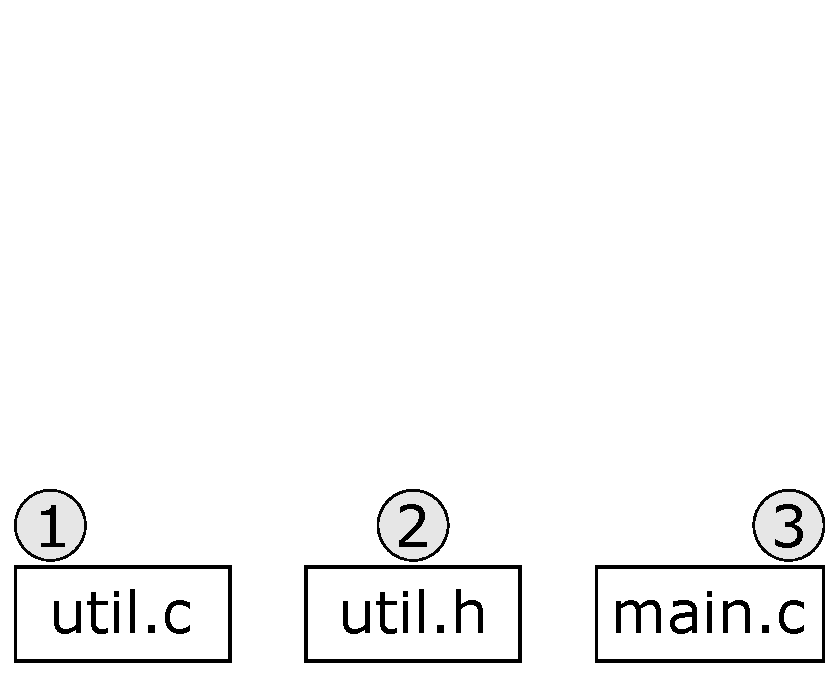
\includegraphics[scale=0.28]{fig/bazel-example-checkout.pdf}}
\caption{Checkout source files}
\end{subfigure}
\begin{subfigure}[b]{0.40\linewidth}
\centerline{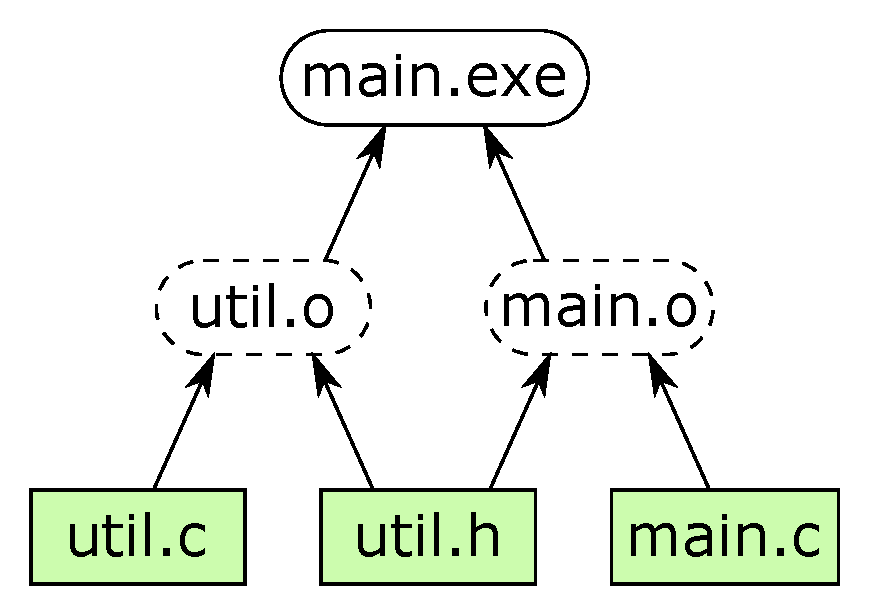
\includegraphics[scale=0.28]{fig/bazel-example-build.pdf}}
\caption{Build \cmd{main.exe}}
\end{subfigure}
\begin{subfigure}[b]{0.31\linewidth}
\centerline{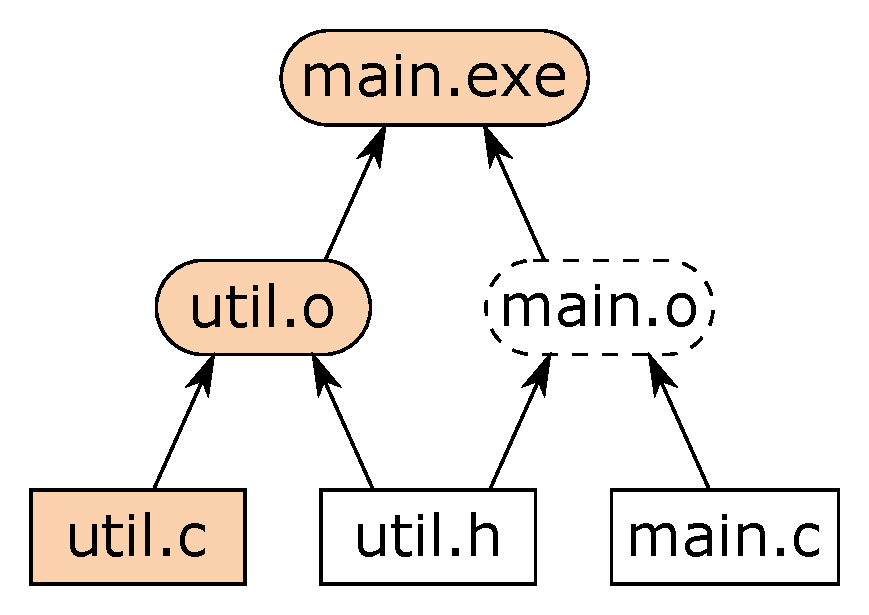
\includegraphics[scale=0.28]{fig/bazel-example-rebuild.pdf}}
\caption{Modify \cmd{util.c} and rebuild}
\end{subfigure}
\caption{A cloud build example: (a)~checkout sources, (b)~download \cmd{main.exe}
from the cloud and skip intermediate files (only their hashes are needed),
(c)~modify \cmd{util.c} and rebuild \cmd{main.exe}, which requires building
\cmd{util.o} (since nobody has compiled \cmd{util.c} before) and downloading
\cmd{main.o}. File hashes are shown inside circles.
\label{fig-bazel}}
\end{figure}

\subsection{Summary}
\label{sec-background-summary}

We summarise differences between four discussed build systems in
Table~\ref{tab-summary}. The column \emph{`persistent build information'} refers
to the information that build systems persistently store between builds:
\begin{itemize}
    \item \Make stores file modification times, or rather, it relies on the file
    system to do that.
    \item \Excel stores one dirty bit per cell and the calculation chain from
    the previous build.
    \item \Shake stores the dependency graph discovered in the previous build,
    annotated with file content hashes for efficient checking of file changes.
    \item \Bazel stores all dependency graphs discovered in previous builds
    annotated with file hashes, and the content-addressable cache.
\end{itemize}

\begin{table}[h]
\smaller
\centering
\begin{tabular}{l||l|l||l|c|c|c}
\hline
$\!$Build system$\!$& Persistent build information   & Algorithm    & Dependencies & Minimal & Cutoff & Cloud$\!$\\\hline
$\!$\Make       $\!$& File modification times        & Topological  & Static       & Yes     & No     & No   $\!$\\
$\!$\Excel      $\!$& Dirty cells, calculation chain & Reordering   & Dynamic      & No      & No     & No   $\!$\\
$\!$\Shake      $\!$& Previous dependency graph      & Recursive    & Dynamic      & Yes     & Yes    & No   $\!$\\
$\!$\Bazel      $\!$& All dependency graphs, cache   & Topological  & Static       & Yes     & Yes    & Yes  $\!$\\\hline
\hline
\end{tabular}
\vspace{0.5mm}
\caption{Summary of build system differences.\label{tab-summary}}
\vspace{-6mm}
\end{table}

In this paper we elucidate which build system properties are consequences of
specific implementation choices (metadata and algorithm), and how one can obtain
new build systems with desired properties by recombining parts of existing
implementations. As a compelling example, we demonstrate how to combine the
advantages of \Shake and \Bazel in a cloud build system with dynamic
dependencies, see~\S\ref{sec-implementation-cloud}.
